\chapter{実験}
\section{実験環境}
実験はシミュレータ上で行い,
シミュレータ環境としてオープンソースの3DロボットシミュレータGazebo\cite{gazebo:online}を用いる.
使用機体についてはturtlebot3\_waffle\cite{turtlebot3:online}へカメラを3つ追加したモデルを使用する.

\begin{figure}[H]
    \centering
    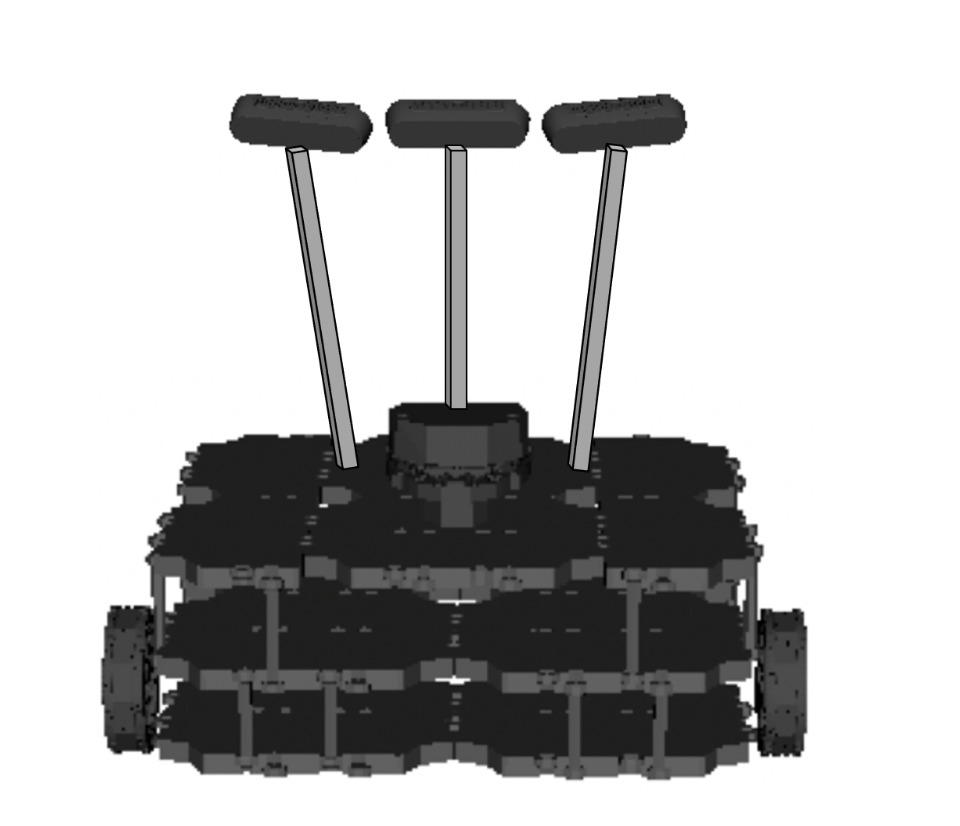
\includegraphics[width = 10cm]{./figs/3_camera.png}
    \caption{turtlebot3 waffle}
    \label{fig::turtlebot3}
\end{figure}

\section{実験方法}

実験における手順を下記に示す
\begin{enumerate}
  \item 学習フェーズを行い,学習器の訓練(経路の学習)行う 
        
  (制御:地図べースの制御器の出力)
  \item 設定したstep数を学習後,訓練フェーズへ移行 
  
  (制御:学習器の出力)
  \item コース内に設定した地点において目標方向のコマンドを入力,挙動を確認
\end{enumerate}
実験はコース内に設定した地点ごとにコマンドの入力による挙動の確認を5回ずつ行う. 
  また,用いるコースは実験ごとに異なるものを用いる.

\section{成功失敗条件}
実験の評価条件を下記のように定義する

成功:分岐路において壁に衝突せず,コマンドに対応したコースを選択

失敗:コマンドとは異なったコースを選択する,分岐路において壁に衝突

\newpage
\section{実験1 十字路}
\subsection{実験目的}
提案手法を用いて,分岐路においてコマンドによってルートの変更が可能であるかの検証を行う.
\subsection{実験環境}
Fig. \ref{fig::zyuzi}に示す道幅が2.5m幅の十字路の環境を用いる.
\begin{figure}[ht]
    \centering
    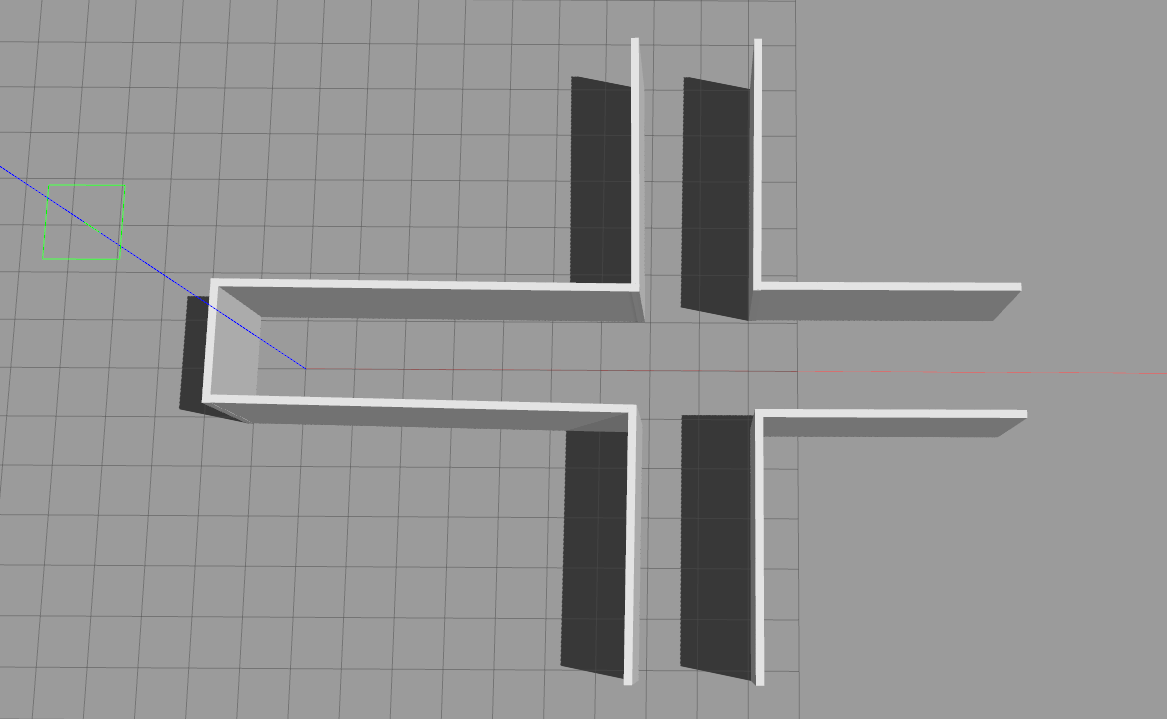
\includegraphics[width = 10cm]{./figs/zyuuziyoko.png}
    \caption{Experiment1 Course}
    \label{fig::zyuzi}
\end{figure}

\newpage
\subsection{学習フェーズでの経路}
学習時の経路についてFig. \ref{fig::exp1route}に示す
Fig内の緑で示す箇所が初期位置,赤で示す円が目標地点である
目標地点を1,2,3の順で走行し,到達後初期値点へロボットの位置,姿勢をリセットする.

\begin{figure}[ht]
    \centering
    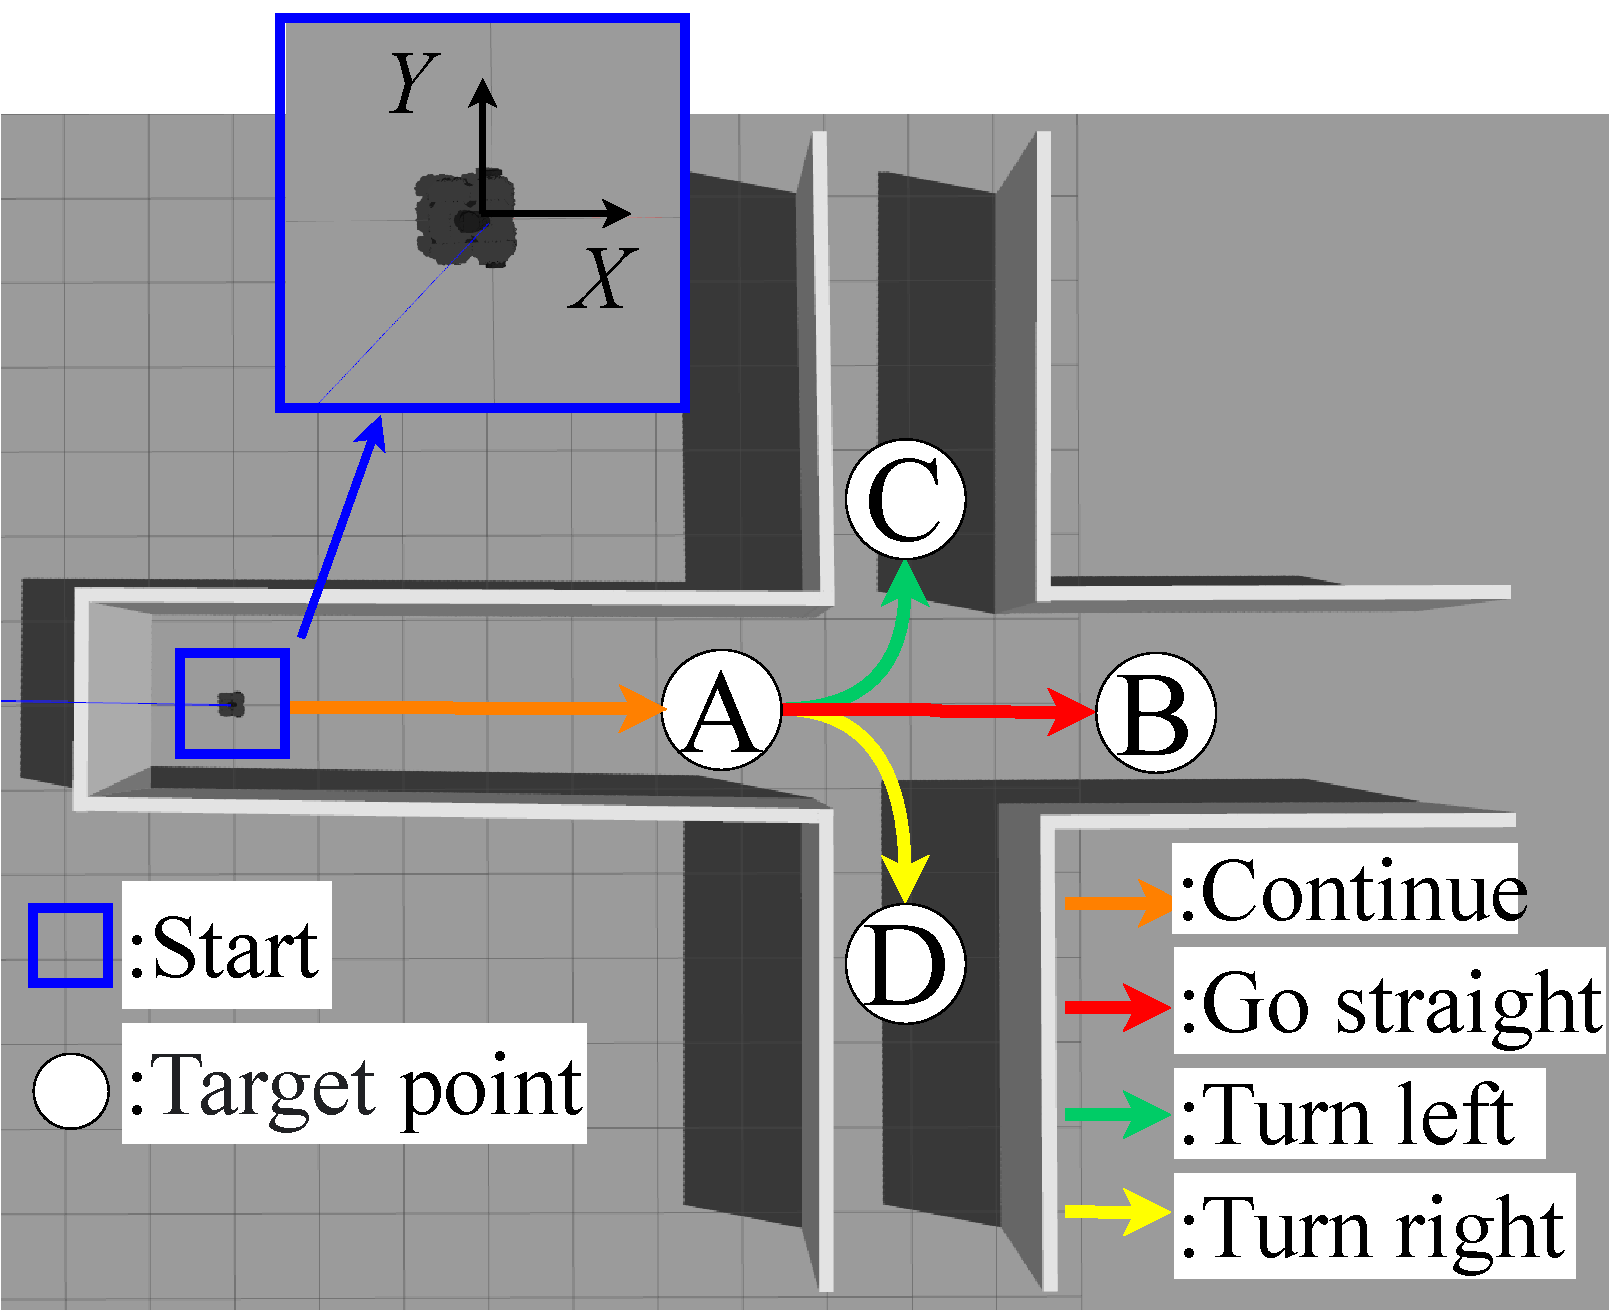
\includegraphics[width = 10cm]{./figs/zyuziroute.pdf}
    \caption{Experiment 1 Route}
    \label{fig::exp1route}
\end{figure}

\subsection{評価}

Fig. \ref{fig::exp1route}で青で示した地点において,
コマンドを入力を行った結果をTable. \ref{tb::exp1suc}に示す.
\begin{table}[H]
  \centering
  \caption{Number of successes Experiment 1 point}
  \begin{tabular}{|c|c|}
  \hline
  Point & Number of successes \\ \hline
  1     & /5                  \\ \hline
  2     & /5                  \\ \hline
  3     & /5                  \\ \hline
  \end{tabular}
  
  \label{tb::exp1suc}
  \end{table}

\newpage
\section{実験2 八の字}
\subsection{実験目的}
実験1で用いた局所的な環境を更に複雑な環境へ拡張し,
提案手法を用いて,分岐路においてコマンドによってルートの変更が可能であるかさらなる検証を行う.
\subsection{実験環境}
Fig. \ref{fig::hatinozi}に示す道幅が2.5m幅の八の字型の環境用いる.
\begin{figure}[h]
    \centering
    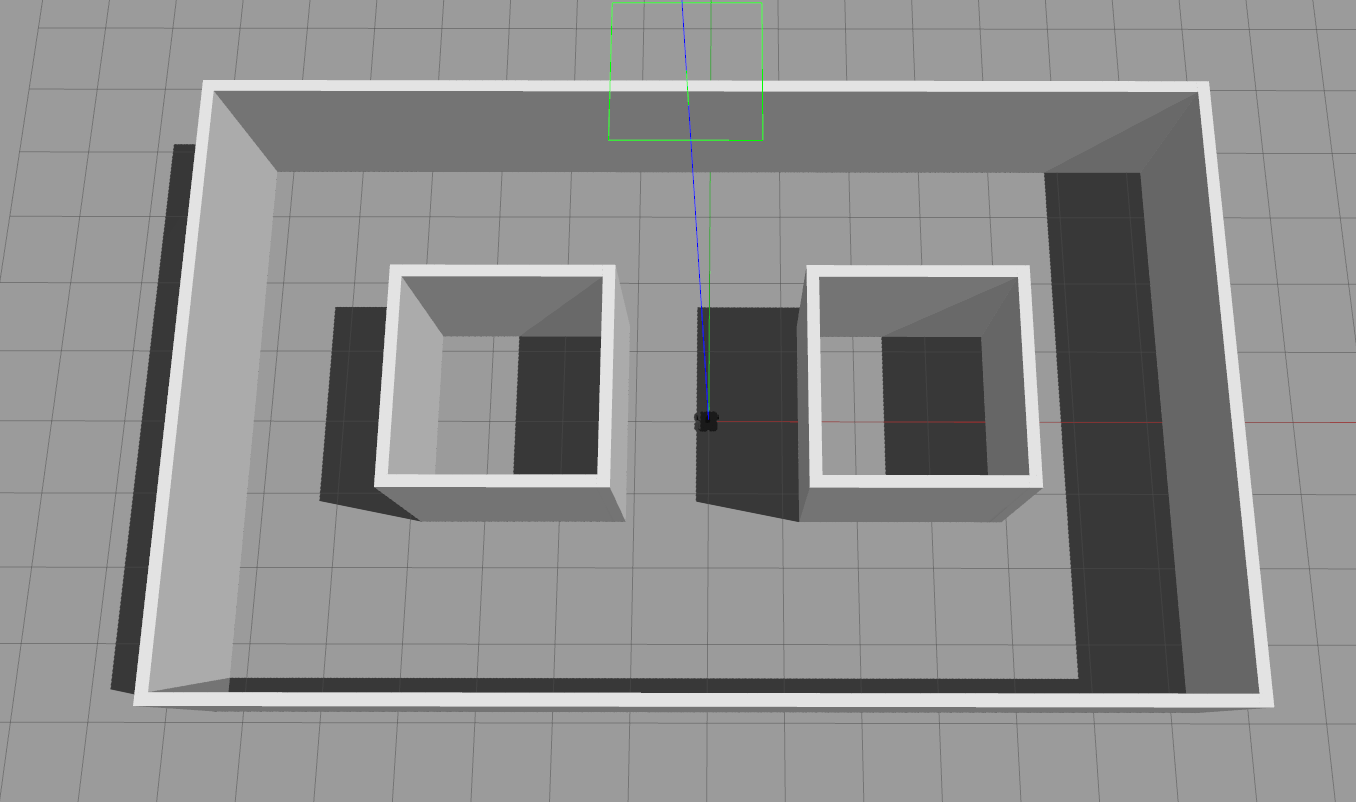
\includegraphics[width = 10cm]{./figs/coli.png}
    \caption{Experiment2 Course}
    \label{fig::hatinozi}
\end{figure}

\newpage
\subsection{学習フェーズでの経路}
学習時の経路についてFig. \ref{fig::exp2route}に示す.
1~6のルートを繰り返し周回する.

\begin{figure}[H]
    \begin{tabular}{cc}
      \begin{minipage}[t]{0.5\hsize}
        \centering
        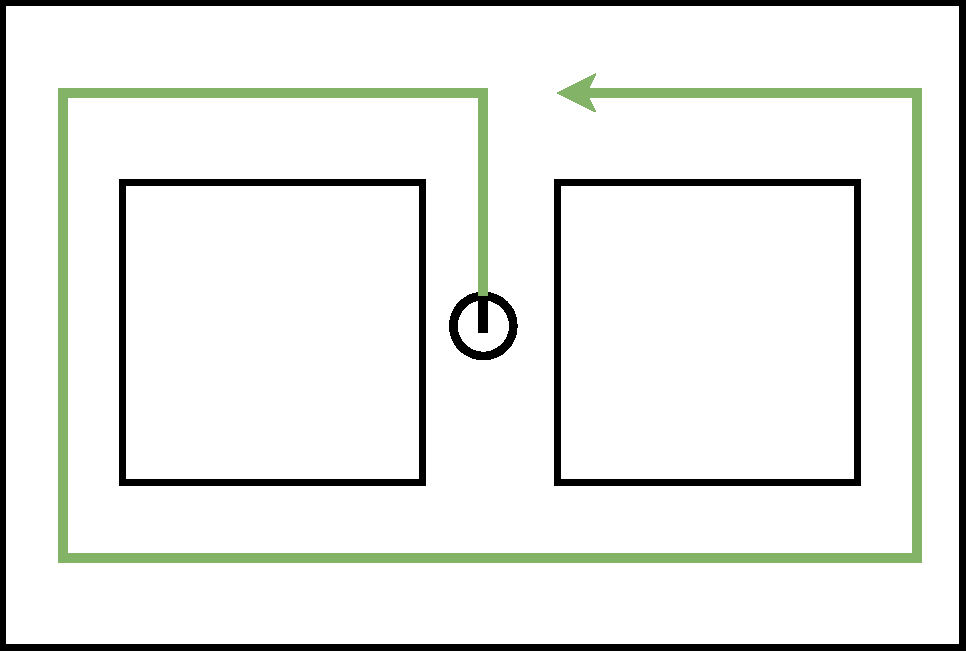
\includegraphics[keepaspectratio, scale=0.4]{./figs/8nozi_1.pdf}
        \subcaption{Route 1}
        \label{exp2route1}
      \end{minipage} 
      \begin{minipage}[t]{0.5\hsize}
        \centering
        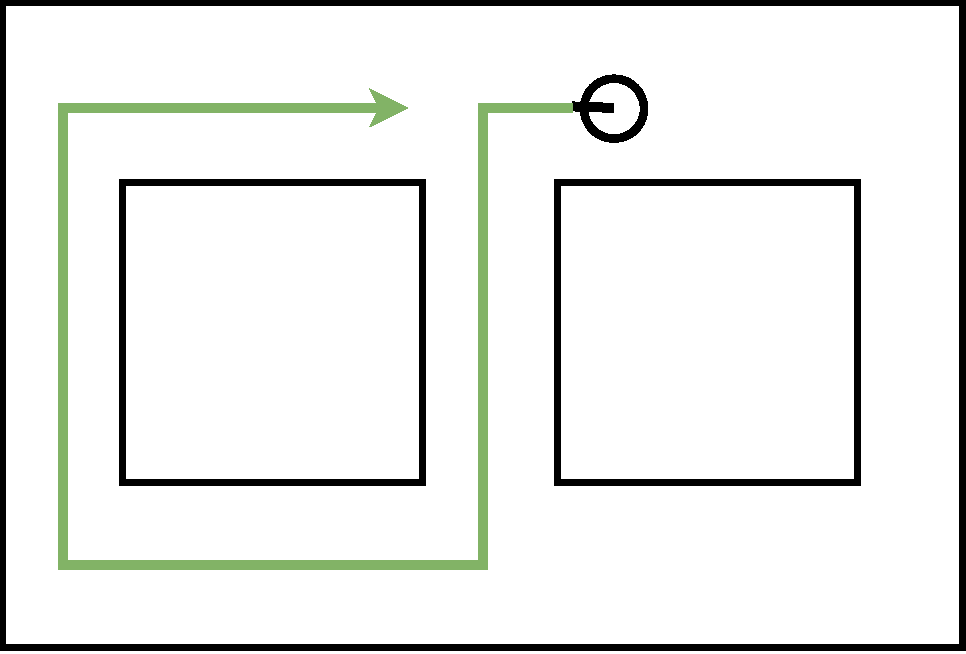
\includegraphics[keepaspectratio, scale=0.4]{./figs/8nozi_2.pdf}
        \subcaption{Route 2}
        \label{exp2route2}
      \end{minipage} \\
      \vspace{2.0zh}
      \begin{minipage}[t]{0.5\hsize}
        \centering
        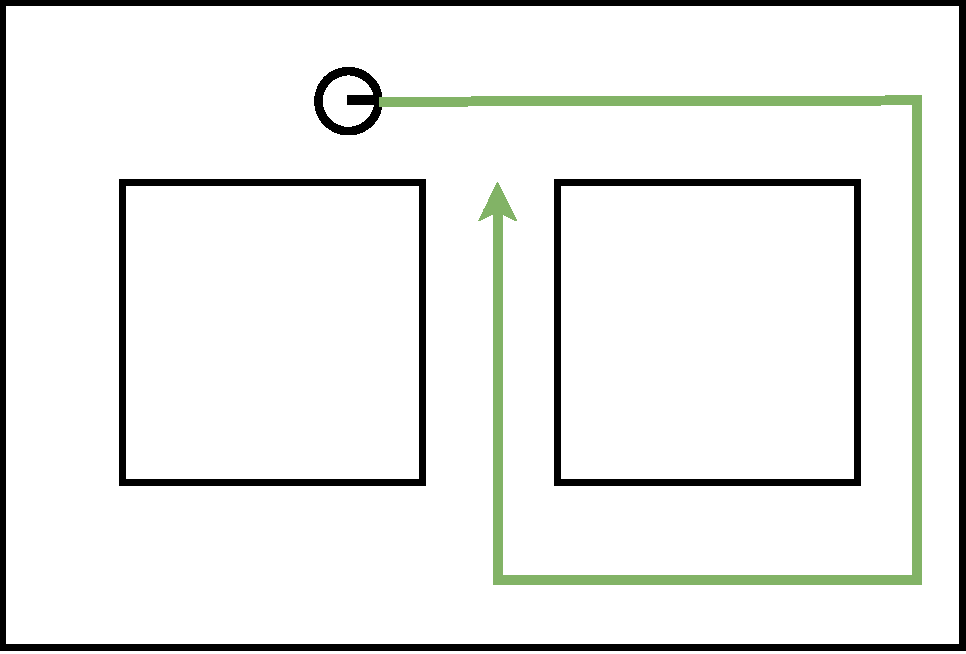
\includegraphics[keepaspectratio, scale=0.4]{./figs/8nozi_3.pdf}
        \subcaption{Route 3}
        \label{exp2route3}
      \end{minipage} 
      \begin{minipage}[t]{0.5\hsize}
        \centering
        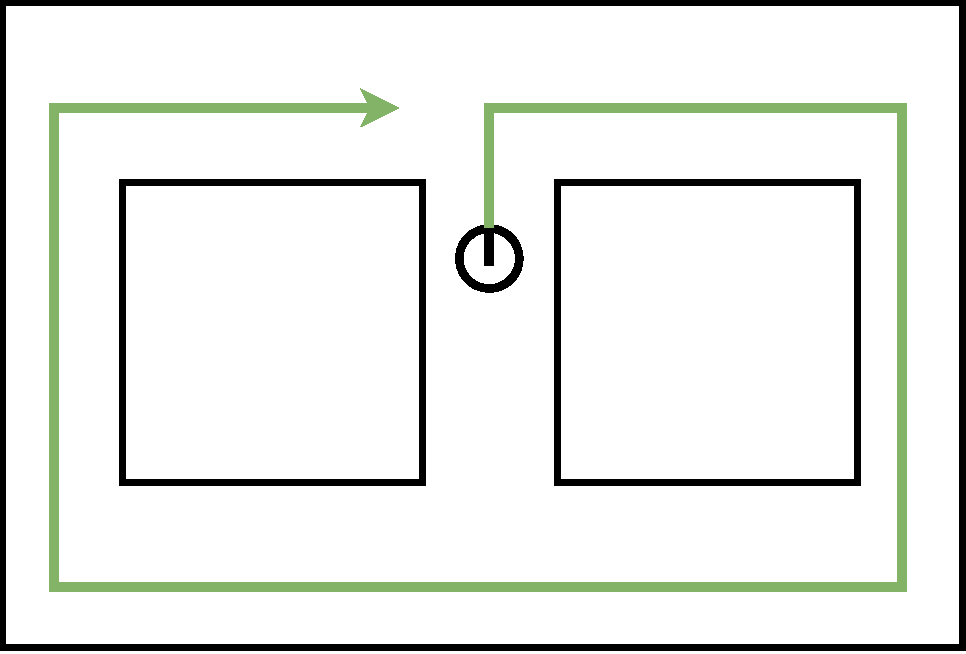
\includegraphics[keepaspectratio, scale=0.4]{./figs/8nozi_4.pdf}
        \subcaption{Route 4}
        \label{exp2route4}
      \end{minipage}\\

      \begin{minipage}[t]{0.5\hsize}
        \centering
        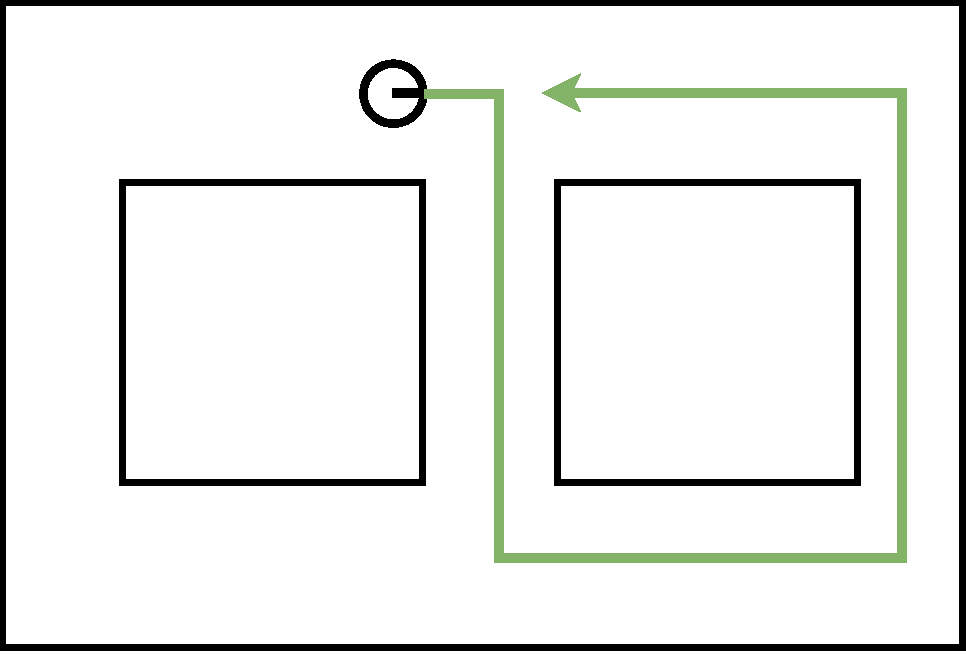
\includegraphics[keepaspectratio, scale=0.4]{./figs/8nozi_5.pdf}
        \subcaption{Route 5}
        \label{exp2route5}
      \end{minipage} 
      \begin{minipage}[t]{0.5\hsize}
        \centering
        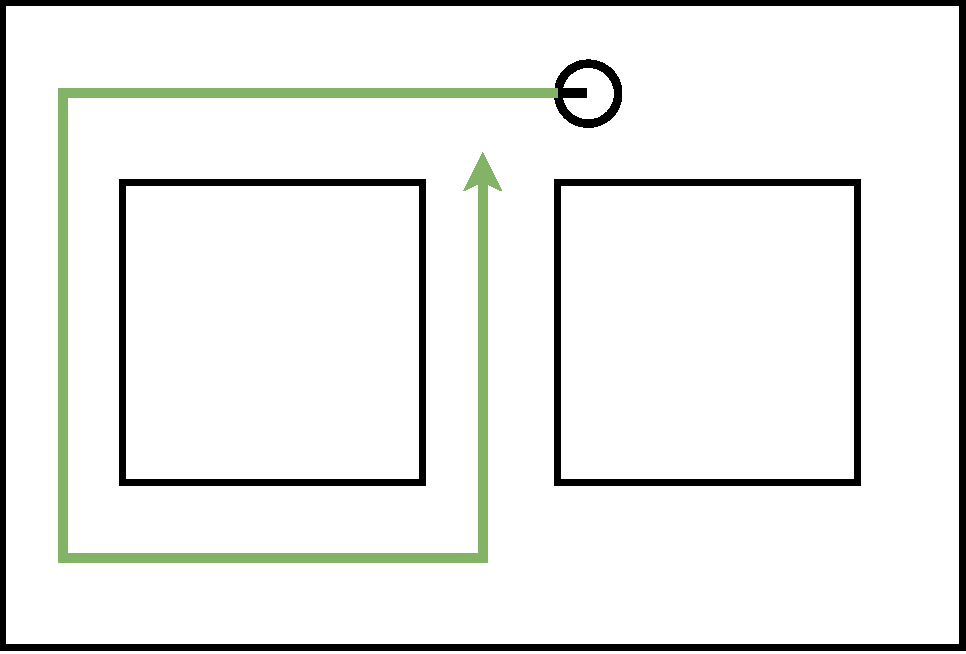
\includegraphics[keepaspectratio, scale=0.4]{./figs/8nozi_6.pdf}
        \subcaption{Route 6}
        \label{exp2route6}
      \end{minipage} 
    \end{tabular}
     \caption{Experiment 2 route}
     \label{fig::exp2route}
  \end{figure}
  
\newpage
\subsection{評価}
コース内の各地点へFig. \ref{fig::bunkiban}で示すように番号をふり,地点ごとの成功回数を
Table. \ref{tb::exp2suc}に示す.
\begin{figure}[h]
  \centering
  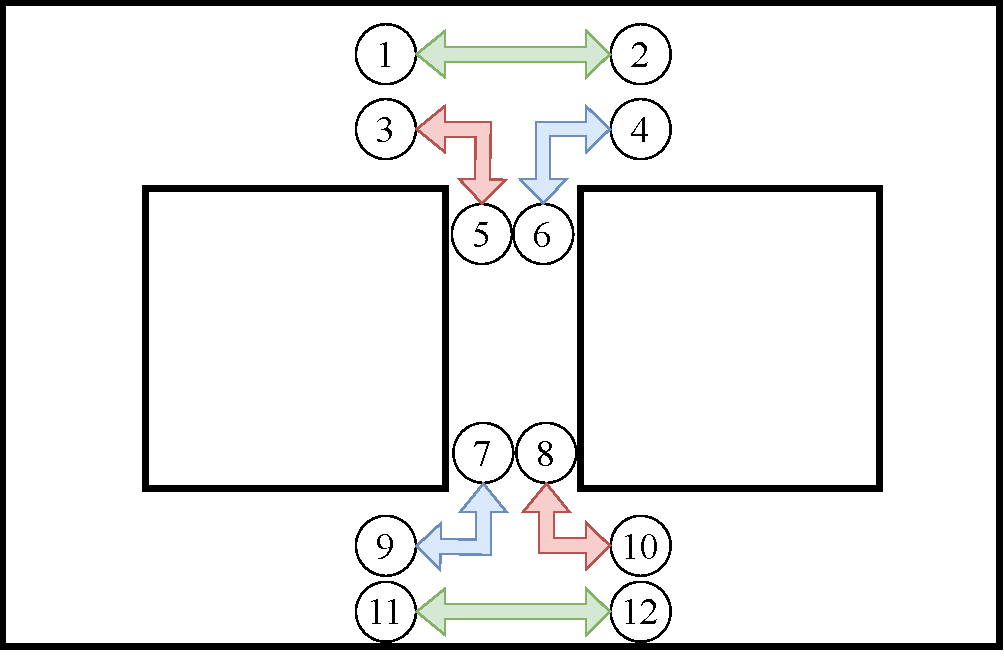
\includegraphics[width = 10cm]{./figs/bunkiban.pdf}
  \caption{Experiment 2 point number}
  \label{fig::bunkiban}
\end{figure}


\begin{table}[H]
  \centering
  \caption{Number of successes Experiment2 point}
  \begin{tabular}{|c|c|}
  \hline
  Point & Number of successes \\ \hline
  1     & /5                  \\ \hline
  2     & /5                  \\ \hline
  3     & /5                  \\ \hline
  4     & /5                  \\ \hline
  5     & /5                  \\ \hline
  6     & /5                  \\ \hline
  7     & /5                  \\ \hline
  8     & /5                  \\ \hline
  9     & /5                  \\ \hline
  10    & /5                  \\ \hline
  11    & /5                  \\ \hline
  12    & /5                  \\ \hline
  \end{tabular}
  
  \label{tb::exp2suc}
  \end{table}
  
% \newpage
% \section{実験3 千葉工業大学津田沼校舎2号館3階}
% \subsection{実験環境}
% 〜に示す道幅が2.5m幅の八の字型の環境用いる.
% \subsection{実験目的}
% 実環境に近い環境で実験を行う
% \subsection{学習フェーズでの経路}
% 蟹